\documentclass{acm_proc_article-sp}

\usepackage[dvips]{graphics}
% pdftex

\pagenumbering{arabic}

\begin{document}

%\setpagenumber{50}

\title{Konfidi:\titlenote{\textit{Konfidi} is the Esperanto term for trust.  
A universal concept in a universal language seemed appropriate for what we hope will become a universal system.} Trust Networks Using PGP and RDF}

\numberofauthors{2}

\author{
\alignauthor Dave Brondsema\\
       \affaddr{Calvin College}\\
       \affaddr{3201 Burton St., SE}\\
       \affaddr{Grand Rapids, MI 49546}\\
       \email{dave@brondsema.net}
\alignauthor Andrew Schamp\\
       \affaddr{Calvin College}\\
       \affaddr{3201 Burton St., SE}\\
       \affaddr{Grand Rapids, MI  49546}\\
       \email{schamp@gmail.com}
}

\date{4 May 2005}

\maketitle
\begin{abstract}
We ought to write this last.
\end{abstract}

\terms{source, sink, concatenation, aggregation}

\keywords{Semantic Web, trust network, FOAF, RDF, PGP, GPG, reputation, propogation, distributed, inference, delegation, social network}

\section{Introduction}
As more and more information becomes available on the internet, there is a growing problem determining which information is reliable and accurate.  A person may, over time, develop a reputation in a certain community as a reliable source of information for a certain topic, however, someone outside that community will likely be unfamiliar with that reputation, and so may not know how much trust she should have in that person.  

Ratings system for reputation within certain domains (eBay auctions, for example), may be of some limited use.  However, unless some there is a system to verify the raters, they may be susceptible to manipulative ratings.  Even if such systems can be guarded against such attacks, why should someone base whether they trust another person on opinions given by others that they neither know nor trust?

One solution growing in popularity is that of creating a network of trust between individuals who know one another and have good reason to trust their estimations of others.  However, these systems too can subject to problems; suppose someone impersonating a trusted party provides incorrect data boosting the reputation of an untrustworthy party.  The Pretty Good Privacy (PGP) encryption system has developed a web-of-trust which can help provide verification of an individual's identity; however, it does not allow the expression of any additional information about that individual's trustworthiness on matters other than personal identification.

In this paper, we will describe some difficulties in integrating reputation-based trust networks with the PGP web-of-trust, and how it might be possible to overcome them.  We will then describe our structure for representing trust data, and our methods for making trust inferences on this data.  Finally, we will discuss the our proof-of-concept software for putting this trust to use.

\section{Related Work}
% do we really need to cover OWL, FOAF, The Semantic Web, wotsap, here?  They are more like building blocks that we can talk about in the relavant subsections of Konfidi
% I think, by specifying them here, we can help keep those sections to a reasonable size

\subsection{Representing Trust Relationships}
There seems to be a general lack of psychological research on ways of representing trust relationships and procedures for making inferences for unspecified relationships. In fact, most work in the fields of mathematics and computer science seems to adopt an arbitrary model appropriate to the algorithm under consideration. As Guha points out\cite{guha04propagation}, there are compelling reasons for a trust representation scheme to express explicit distrust as well as trust.

% we should talk about this later, if at all
%For Konfidi, we have likewise has chosen an arbitrary model, but in designing the system we have made every effort to allow for adaptation to different models as research in this area develops. 

\subsection{Trust Networks and Inferences}
There are a number of papers about different propagation strategies for weighted, directed graphs\footnote{See such-and-such, and so-and-so, for example}.  For the most part, however, they are concerned with describing the networks mathematically, and do not have much in the way of practical application.  While they are of interest and relevance, they concern only the subsystem and do not discuss the design of a larger infrastructure.

Jennifer Golbeck, at the University of Maryland, is doing graduate research on trust and reputation systems\cite{golbeckSite} that is similar to our work on this project.  Like us, she uses an extension of FOAF to represent trust relationships and a rating system\footnote{Though both our ontologies and are ratings are different in significant ways, which we will address later.}.  She has written a number of papers and created TrustMail\cite{trustMail}, a modified email client that uses the trust network that she is building.  She is more concerned with an academic approach than a pragmatic one, since this field is still growing rapidly and she prefers to help research other applications and implications of semantic social networks.

Golbeck suggested an important distinction between belief in statements and trust in people\cite{golbeck:accuracy}.  While networks of both kinds can be created, the latter are usually smaller and more connected.  Golbeck argues that using a network of trust in people is equivalent to one of belief in statements and allows for simpler traversal.
% What about the issue of statements about yahoo.com.  How could a person-only network be equivalent?)

\subsection{The Semantic Web}
In addition to Golbeck's work, a number of others have explored the usefulness and implications of expressing trust relationships in the Semantic Web.

\subsubsection{Friend of a Friend (FOAF)}
\label{foaf}
The FOAF project\cite{foafProject} is a Resource Description Framework (RDF) vocabulary used to represent personal data and interpersonal relationships for the Semantic Web.  Users create RDF files describing Person objects which can specify name, email address, and so on, but more importantly, they can express relationships between Person objects.  There are a number of tools in development for processing FOAF data and traversing references between FOAF RDF files.  These tools can aggregate information because RDF often uses uniform resource indicators (URIs) to describe an individual object.

\subsubsection{FOAF Whitelisting}
Dan Brickley has made a practical attempt to investigate the use of FOAF, particularly the mbox\_sha1 property, to automatically generate email whitelists. By hashing the sender's address using SHA1, privacy is protected (and the address cannot be gathered by spiders), and so users can share whitelists of non-spam emailers. Then for all incoming mail, the sender's address is hashed and the whitelist searched for the resulting value, and then is filtered accordingly. This use of FOAF is promising, but since it is decentralized, it is difficult for updates to propagate\cite{foafWhitelisting}. No effort was taken in this project to verify the sender's identity.

\subsection{Email Filtering}
Filtering email to reduce unsolicited email has received lots of attention in many areas.  Domain-level solutions, such as SPF and DomainKeys, are mostly to prevent phishing and also assume that a domain's administrator can control and monitor all its user's activities. Greylisting and blacklisting often have too many false positives and false negatives. User-level filtering, which Konfidi does in the context of email filtering, is not very common. Challenge-response mechanisms to build a whitelist are tedious for the sender and reciever and do not validate authenticity. Content-level testing is the most common, but bayesian filtering and other header checks are reactionary and must be continuously updated, and are becoming less effective as spammers create emails that look more and more real. 

\subsubsection{Inferred Trust}
Boykin and Roychowdhury discuss ways to infer a relationship based on existing data\cite{boykin04email}.  They suggest scanning the \texttt{From:}, \texttt{To:} and \texttt{Cc:} headers and building a whitelisting database based on relationships indicated by the recipients.  This seems to work fairly well, but there is often not enough data to make the spam/not-spam decision because it is based only on the user's own previously received messages. They clearly state a cryptographic solution would be ideal to verify identity.

\subsection{Trust Inference Using PGP}
\label{earlierPGP}
One possible approach\footnote{This is the basis of our approach with Konfidi} is to use the PGP web-of-trust to filter email spam at the client's end. For example, a mail client plugin could filter incoming mail, and attempt to find a path from the sender to the recipient\footnote{In the web-of-trust, nodes are PGP keys and edges are key signatures.  Paths are made when the recipient had signed someone's key, who had signed another key, and so on until a signature is found on the sender's key}. If a path could be found under a specified length, the message would be marked as trusted.  Otherwise, it would be marked as not trusted. This approach requires that most users digitally sign email messages, and it depends on users to be aware of known spammers and avoid signing their keys. However, the recommended PGP keysigning practices require only the careful verification of the key-holder's identity, and a signed key does not entail anything about trustworthiness in other areas.  Furthermore, if the identification requirements for keysigning are met, even by a spammer, it would be unfair to refrain from signing that spammer's key\footnote{In fact, such positive identification might be of use.}.  Whether a user should be trusted to send good email, and not spam, is information over and above that expressed in the PGP web-of-trust itself, so the web-of-trust would be inadequate to encode such information.

A more serious flaw in this approach is this:  because information about key signatures is stored with the key that was signed, and not that of the signer, paths between users can only be constructed from the sender backward to the recipient. When a key is retrieved from a keyserver, all of the signatures on that key are included with it, showing which keys have signed that key, and providing a number of possible links in a chain. However, using the existing keyserver infrastructure without a transformation of some kind, there is no easy way to tell which other keys a particular key has signed. If these paths are built backward using a breadth-first search from the sender to the recipient, a spammer or other malicious user could generate a large number of fake keys that are inter-signed, and then use these keys to sign the sender's key. By adding this artificial information, the client's searching capabilities would be crippled, and the web-of-trust would be filled with fabricated keys, users, and signatures, quickly becoming useless. The PGP system of key-signing and verification was designed to be robust against this sort of impersonation, by requiring photo-identification and fingerprint exchange before any key-signing, but a deluge of false information would put undue strain on the keyserver infrastructure, and would amount to a denial-of-service, of sorts.

\subsubsection{Wotsap}
\label{wotsap}
% what should we say here, dave?
Talk about wotsap a bit.

\section{Motivation/Desiderata}
% I asked Vlinden about this, but no response yet.
So, for our idea to be viable, it must first deal with these two issues, namely, representing trust information not directly in the PGP web-of-trust but rather in some other system closely coupled with it, and not being susceptible to denial-of-service attacks caused by generated false webs. We had other requirements, too. A system like this must be widely (even universally) adopted in order to be useful. As such, it must be easy for the technically unsavvy, like Aunt Sally, to use, while at the same time avoiding any diminished security stemming from being easy-to-use. It must also be available in any of the many widely-used email clients. 

\section{Konfidi}

Konfidi refers to the trust network design, the ontology used to encode it, and the software to make it usable.

\begin{figure*}
\centering
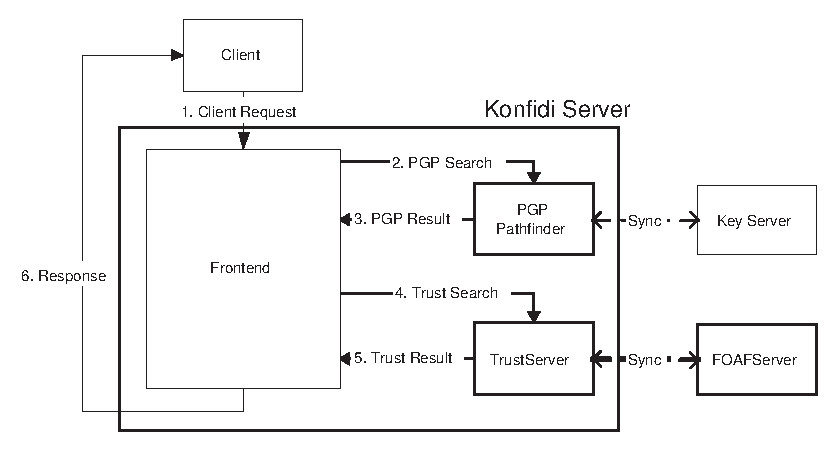
\includegraphics{arch.eps}
\caption{The Konfidi Architecture}
\label{fig:Arch}
\end{figure*}
\subsection{Trust Ontology}
% representation is seperate from algorithm result, right?  Need to fix this paragraph if so
% what do you mean?  I suppose the algorithm can perform whatever operation on the values it wants, but I think the point is that the domain and range of the network is the same:  an inferred trust rating should look no different from an explicit one.  maybe this is unclear...
% Right.  Then with discrete values for levels of trust, the output should be one of those discrete levels, not a binary yes/no.  The binary yes/no is a client threshold decision that would be done for both continuous and discrete outputs.
In the current research on trust inference networks, there seem to be two general kinds of representations:  one that used discrete values for varying levels of trust and returned a discrete binary (yes or no) answer, or one which used a (theoretically) continuous range of trust values and returned an answer within that range.  Now, either kind of representation could be roughly mapped onto the other, however, a continuous range would allow more finely-grained control over the data.  Further, the inferred trust values returned by searches would be similar to the explicit trust values users provided when specifying trust relationships.  This makes it easier to evaluate such results on a scale that has some familiarity.

\subsubsection{Distrust}
The choice of representation is closely related to another important concern, that the representation give some account of distrust.  If the trust network contained values ranging from neutral trust to complete trust, then everyone in the network is trusted, explicitly, or by inference on some level at or above neutral.  If the system makes a trust inference between Alice and Bob at one level, but Alice really trusts Bob at a different level, she can explicitly state this previously implicit trust to have a more accurate result (for herself and for others who build inference paths of whom she is a member).  But, suppose that Alice feels strong negative feelings about Bob.  In this case, she would still only be able to represent this relationship as one of neutral trust.  So, the trust network must account for distrust in some reasonable way.
% refer to samples from diagram

One of the difficulties of using explicit distrust in an inference network, however, is that it is unclear how inferences should proceed once a link of distrust has been encountered.  Suppose Alice distrusts Bob, and Bob distrusts Clara.  As Guha points out\cite{guha04propagation}, there are at least two interpretations of this situation.  On the one hand, Alice might think something like "the enemy of my enemy is my friend" and so decide to put trust in Clara.  On the other hand, she might realize that if someone as scheming as Bob distrusts Clara, then Clara must really be an unreliable character, and so decide to distrust Clara.  Further, suppose Bob expressed trust for Dave.  At first consideration, it might seem reasonable to simply distrust everyone that Bob distrusts, including Dave.  But suppose there were another path through different nodes indicating some minimal level of trust for Dave.  Which path should be chosen as one which provides the correct inference?

One solution to this problem is simply to not traverse beyond a relationship of distrust, and to seek an alternate path.  There is no clear answer regarding the statements a distrusted person makes, so it is best not to consider them at all.
% multiple paths is different than distrust.  Move the following elsewhere
To overcome the problem of chosing the correct path for the inference, some kind of weighted average can be taken of all of the paths between Alice and Dave, thereby producing an answer according to whether the majority of people in the neighborhood Dave trust him or not.

We explored a method similar to this one, but in the absence of sufficient psychological research affirming a model of this type, we sought a simpler solution.  In the end, we decided on a model that corresponds to another intuition about how trust works between people, that it is more of a continuum of both trust and distrust than a measure of just one or the other.  For example, if Alice trusts Bob at some moderate level (say, .75 of a scale of 0 to 1), then it seems that she also \textit{distrusts} him at some minimal level (say, .25).  If Alice trusts Bob neutrally, then she trusts him about as much as she distrusts him.  If she distrusts him completely, then she doesn't trust him at all.  But in all of these cases, there is a trade-off between trust and distrust.  Only in the extremes is either of them eliminated completely.  So, we decided that our trust model should represent a range of values from 0 to 1, treating 0 as complete distrust, 1 as complete trust, and 0.5 as neutral, and calculate trust inferences accordingly\footnote{This also makes many propagation algorithms simpler, as we'll discuss later.}.

\subsubsection{Trust Topics}
If other attributes about a trust relationship could be expressed, in addition to the rating system, then a system like Konfidi would be useful in many wider scopes than email spam prevention.  The most important of these is the trust topic, or in other words, what the trust is about.  A natural feature of interpersonal trust relationships is that there can be many different aspects of the same trust relationship.  

(you can make an Alice-Bob-Clara-Dave diagram for this business)

For example, suppose Bob is a master chef, but is terribly gullible about the weather forecast.  Alice, of course, knows this, and so wants to express that she trusts Bob very highly when he gives advice for making souffle, but she does not trust him at all when he volunteers information about the likelihood of the next tornado.  Suppose she only knows Bob in these two capacities.  Any trust inference system should not average the two trust values and get a somewhat neutral rating for Bob, for that would lose important information about each of those two trust ratings\footnote{In fact, it would lose the only information that made these ratings useful in the first place.}.

Suppose also that, given only the above trust ratings, the system tried to make an inference on a subject that was not specified.  Perhaps Alice has some general level of trust for Bob that should be used when there is no specific rating for the topic in question.  See the discussion in Future Work for our proposal for a hierarchical system of topics that might account for this situation.

\subsubsection{Rating Values}
\label{rating}
% "Rating System" seems inappropriate.  How about "Data structure" or something?
% how about "rating values?"
% the first half of this paragraph is about the relationship-based model, the second half is about the ratings, and the 2nd paragraph is about attributes.  We need a more general title if we're going to have all these concepts in one section
With these considerations in mind, we found that a relationship-based model would meet our needs while avoiding some of the disadvantages of other representations.  According to this system, each trust relationship is an object, and the trusting person and the trusted entity (typically a person) are specified as such\footnote{Thus, each relationship is one-way, but since the truster is responsible for the accuracy of the information, that is fine.}.  Trust relationships also have trust items specified.  Each item is composed of a topic and a numerical rating.  Each rating is on a scale from 0 to 1 inclusive, with 0 representing complete distrust, 1 representing complete trust, and 0.5 representing neutral.

Because the trust relationship is represented as its own object, other attributes may be added later, such as the dates the relationship began, annotations, etc. as the need arises.

\subsubsection{OWL Schema}
As the FOAF project grows in popularity, an infrastructure is growing to support it, as mentioned in \ref{foaf}.  Since there would be many advantages to tapping into this infrastructure, and since the specification of trust relationships fits in naturally alongside the existing \texttt{foaf:knows} property, Konfidi also uses the Resource Description Framework (RDF)\cite{rdf} for representing trust relationships.  In addition to the FOAF vocabulary, there is a vocabulary called WOT defining and describing singing and assurance, which provides the necessary structure for associating persons and organizations with key fingerprints\cite{wot}.  By designing Konfidi's vocabulary to make use of FOAF and WOT vocabulary elements, then, we can take advantage of the established standards and make our extensions compatible with existing FOAF-enabled tools.

Konfidi uses the Web Ontology Language (OWL)\cite{owl} to define the RDF elements that make up the Konfidi trust ontology.  OWL builds on the existing RDF specification by providing a vocabulary to describe properties and classes, and their relations.  The Konfidi trust ontology provides two objects and five properties, which, in conjunction with the existing FOAF and WOT vocabularies, are sufficient to describe the trust relationships that Konfidi requires.

The primary element is \texttt{Relationship}\footnote{According to RDF standards, the names of objects are capitalized, while the names of properties remain lowercase.}, which represents a relationship of trust that holds between two persons.  There are two properties required for every \texttt{Relationship}, \texttt{truster} and \texttt{trusted}, which indicate the two parties to the relationship.  Both \texttt{truster} and \texttt{trusted} have \texttt{foaf:Person} objects as their targets\footnote{These \texttt{Person} objects should also contain at least one \texttt{wot:fingerprint} property specifying the PGP fingerprint of a public key held by the individual the \texttt{Person} describes.  This property is required for verification; if no \texttt{fingerprint} is available, then Konfidi cannot use the relationship.}\footnote{In general, any objected described in RDF with a resource URI can be the \texttt{trusted} party, such as specific documents or websites.  We will focus on persons for simplicity.}, which may be defined in the same file, inline, or in external documents indicated by their resource URIs\footnote{Because it does not matter where the \texttt{foaf:Person} data is stored, users may keep files indicating trust relationships separate from main FOAF files.  However, to prevent spoofing, any file containing one or more \texttt{Relationship} objects must have a valid signature from a public key \texttt{fingerprint} corresponding to each \texttt{Person} listed as a \texttt{truster} in that file.  As described in \ref{foafserver}, flexibility in data location can have a number of advantages. }.  

In addition to \texttt{truster} and \texttt{trusted}, each \texttt{Relationship} requires at least one \texttt{about} property, which relates the trust \texttt{Relationship} to a trust \texttt{Item}\footnote{A \texttt{Relationship} is not limited in the other properties it can have, so auxiliary information about the relationship, such as when it began, who introduced it, etc. may be recorded without having an effect on the requirements of Konfidi.}.  Each \texttt{Item} has two properties belonging to it.  The \texttt{topic} property specifies the subject of the trust according to a trust topic hierarchy\footnote{yet to be developed} and the \texttt{rating} property indicates the value, according to the 0-1 scale of trust (specified in Section~\ref{rating}) that is assigned to the relationship on that topic.  

A \texttt{Relationship} may have more than one \texttt{Item} that it is about.  For example, remember the example given above, in which Alice trusts Bob highly about cooking, and distrusts him somewhat about the weather.  This might be represented in our ontology as something like the following\footnote{That is, supposing that the objects \texttt{alice123}, \texttt{bob1812}, \texttt{cooking}, and \texttt{weather} are all defined elsewhere in the same file.}.  For a more in-depth example, see Appendix~\ref{trustExample}.:

\begin{verbatim}
<Relationship>
  <truster rdf:resource="#alice123" />
  <trusted rdf:resource="#bob1812" />
  <about>
    <Item>
      <rating>.95</rating>
      <topic rdf:resource="#cooking" />
    </Item>
  </about>
  <about>
    <Item>
      <rating>.35</rating>
      <topic rdf:resource="#weather" />
    </Item>
  </about>
</Relationship>
\end{verbatim}

See Appendix~\ref{schemaCode} for the full OWL source code.

\subsection{TrustServer}
This part of the design is the core element of Konfidi.  Storing and managing the data would not be of much use in this context unless we did something with it.  So, the TrustServer would handle requests for trust ratings, verify that a PGP connection exists, and traverse the internal representation to find a path.  Since these three tasks are so distinct, all of Konfidi is divided into three parts, a frontend which listens for requests and dispatches them, and two backend components, one to search the PGP web-of-trust and another to query against Konfidi's own trust network.  This separation, in addition to simpilifying the design by encapsulating the different functions, also allows for increased flexibility and scalability.  Each part is loosely coupled to the other parts, with a simple API for handling communications between them.

\subsubsection{Frontend}
Like the FOAFServer, the TrustServer's frontend is a web service, using the REST architecture to receiving and answering queries. 
%more here tying specifics of REST in as advantages, as outlined in the FOAFServer
It also runs on the Apache web server, using the mod\_python framework.  Queries are passed in using HTTP's GET method, and responses are returned in XML, which a client application may parse to retrieve the desired data.

% this is first use of source/sink.  Might need to explain here or before
When a query is received, the Frontend passes the source and sink fingerprints to the PGP backend, and, if a valid path is found, to the trust backend\footnote{Strictly speaking, either query is optional.  The PGP backend may be skipped to run tests on large sets of sample data, and the trust backend may be skipped if the system is to be used as an interface to the PGP web-of-trust only.}.  The Frontend then builds the response document in XML, and passes the result back to the client\footnote{The client may also request for simplicity a single value, the trust rating value.}.

\subsubsection{PGP Pathfinder}
As mentioned in Section~\ref{earlierPGP}, the PGP web-of-trust is not sufficient for determining trust.  However, it is necessary for the proper operation of Konfidi because it plays a very important role in verifying the identity of the sink.  If the author of a document were not identified correctly, someone might forge the trust data, and Konfidi would return a deceptive result.  Verifying that the document's signing key matches the key of the sink in the Konfidi trust network ensures that when Konfidi finds a topical trust inference path from source to the sink, it is valid.

Since one purpose of Konfidi is to provide trust information over and above the PGP web-of-trust, it may seem natural to keep the Konfidi trust network tightly coupled to it.  In other words, every trust link specified using the Konfidi trust ontology corresponds to a link in the PGP web-of-trust made by signing the appropriate key.  However, there are compelling reasons not to do this.  First, the set of people one might wish to indicate trust for in Konfidi will likely not be the same as the set of those whose keys you are able to sign.  For example, a researcher in Sydney may work closely with another in Oslo, and so trust that person's opinion highly in matters relating to their research.  But unless they are able to meet at a conference some time, or are willing to fly halfway around the world, it is unlikely that they will be able to sign each other's keys directly.  However, a valid path in the PGP web-of-trust may already exist connecting them.

Second, requiring users to sign the key of each person they want to add to their Konfidi trust networks adds additional difficulty which should otherwise be avoided.  In keeping with the recommended practices for PGP, two individuals must meet in person and verify photo identification before they are to sign each other's keys.  This extra hassle might entice users to grow lax in their keysigning policy, failing to properly complete such requirements.  This attitude, when widespread would substantially weaken the web-of-trust.  By keeping the PGP web-of-trust separate from the Konfidi trust network, the strength of the web-of-trust will not be weakened needlessly.

An additional advantage of separating the two trust networks is usability.  Aunt Sally can use Konfidi to indicate trust if she and one other person (say, a more technically savvy nephew) sign each other's keys.  She will then probably be connected to the PGP web-of-trust within a reasonable distance of other family members which she is likely to include in her trust network.  Now there is no need to teach Aunt Sally the requirements for key signing, and explaining why they must be done for each person she wishes to add to her Konfidi trust network.  The system is easier to use, and the web-of-trust is less likely to be compromised\footnote{While the effects of individual keys being compromise on the web-of-trust as a whole would be restricted to the key's neighborhood in the web, as this happened with greater frequency, the usefulness of the entire web would be undermined.}.

%how should I re-introduce this business?
% I respond with another question.  What's the point of this (and the following) paragraph?  What are you trying to achieve?
% we'll take this bit out soon.
%As you remember, before completing a query on the Konfidi trust network, the frontend will verify that a valid path exists on the PGP web-of-trust.  While we are eager to avoid some of the difficulties with searching the web-of-trust using the existing keyserver infrastructure, as mentioned in Section~\ref{earlierPGP}, it was not the main goal of our project to deal with all of them at this stage.  

The frontend uses a number of drivers in a Strategy pattern \cite{designPatterns}, so that different subsystems for doing PGP pathfinding can be interchanged as they are developed.  The current version utilizes a pathfinder known as Wotsap \cite{wotsap}, which downloads the complete web-of-trust from a keyserver and stores it in an intermediate format for searching.
% can you think of something else to say here about wotsap?  like, we're working on a way to make it faster, or it currently is not completely secure.  would this be a good place to mention that all data  and sources must be trusted for the Konfidi trust network itself to be trustable?  how might we go about achieving this?
% or maybe in the end section?

\subsubsection{Trust Backend}
The Konfidi trust backend is responsible for storing the internal representation of the Konfidi trust network, incorporating updates into the network, and responding to queries about the nodes in the network.

The backend can register with a FOAFServer as a mirror to receive notification whenever a FOAF record with trust information is added or altered.  It needn't ever notify the FOAFServer of any updates to its records, for the FOAFServer would be the only source of new information.  This allows also for it to syncronize with the FOAFServer after a period of down time in which new records have been added.  The backend currently assumes that the FOAFServer has verified the signatures of the FOAF records it stores, freeing it from the computational burden of fetching the signing keys and verifying the signature.
% change above?

When the TrustServer updates a record, the backend parses the RDF input data and adds the relevant information to its internal representation of the trust network, which is a list of all \texttt{foaf:Person} records indexed by fingerprint and links to each \texttt{Person} marked as trusted, along with topic and rating data.  The updated data will then be available for subsequent queries.  This scheme accomplishes the goal of having trust links available in the proper direction, from source to sink, and avoiding one species of bogus data attack, as discussed in Section~\ref{earlierPGP}.  

% dave, check this complexity analysis and make sure you agree.  it's important.
This representation requires $O(m+n)$ space to store and on average, $O(m*l)$ time to search, and $O(o+p)$ time to update, where $m$ is the number of persons, $n$ is the number of trust links, $l$ is the average length of a path between two persons, $o$ is the number of persons being updated, and $p$ is the number of links being updated.  On the other hand, a representation of a completely solved network, storing the trust values between any two individuals\footnote{In other words, a lookup table.}, requires $O(m^2)$ space, but makes trust queries take a maximum of $O(1)$ time.  However, such a representation requires $O(m^2*l)$ time to solve, which it must do again after every update, since it must recompute the value for every pair.\footnote{The tradeoff between storage space and query time made it hard to settle on a representation.  Perhaps a compromise between a "live" system that incorporates incremental updates with slow queries, and a system that updates its network several times a day, rather than on each update, could provide better performance.  Most users would not need up-to-date links with every user, since their queries would most likely be over a rather limited subset of the network.  Caching of previously computed trust values on the user's end, with periodic updating, could also make a difference.}

It may also be advantageous to store trust links going the other direction, perhaps for local representation analysis, or auxiliary information like name or email address.  Other information, such as when the record was last updated, could allow for record caching that might improve performance.

Because of the apparent lack of psychological research on trust representations, we have again implemented the Strategy pattern\cite{designPatterns}, for the trust propagation algorithm.  This allows additional propagation strategies to be dropped into place as they are developed.\footnote{It also served, unlooked for, as an excellent interface for various special queries we wanted to make, like getting a list of all the people in the network, or a full dump of all people and trust data.}  Our preliminary algorithm does simple multiplicative propagation over each link in a path.  It uses something like a breadth-first search\footnote{Prioritized to follow whichever path has highest value after each iteration.} to find the shortest path between source and sink, if one exists:

\begin{verbatim}
function findRating(source, sink):
  keep a priority queue of all paths
  until the sink is found
    find the path with the highest rating
    find the link not already seen
      concatenate ratings from path and link
      add the path with its rating to the queue
  return the rating of the path to the sink
\end{verbatim}
% sentence may be interpreted as "return (the rating of the path) to the sink"

One such concatenation algorithm is a simple strategy like the following, which simply multiplies trust ratings along each step in the path:

$r = \prod_{i=0}^{n-1} Rating(i, i + 1)$

where $Rating$ returns the rating between two nodes in the network.

\section{FOAF Server}
\label{foafserver}
% in the "owl schema" section, I say that this section talks about the advantages of having distributed FOAF and RDF records, so be sure to cover that here as part of hte motivation of the Foafserver.  you remember what I mean, right?

The Konfidi server uses data from PGP keyservers to act on identity trust.  To act on topical trust, we need a similar data store.  This is not necessarily within the scope Konfidi, but is a necessary prerequisite.  We created the FOAF Server to fulfill this need.

The FOAF Server is a web service that stores and serves FOAF files that include trust relationships as specified by our trust ontology.  A seperate FOAF file is stored for each person, identified by their PGP fingerprint.  All FOAF files must be PGP signed by the owner to prevent false data from being submitted and to prevent unauthorized modification of someone else's data.  When a FOAF file is requested, the PGP signature is included also so that it may be verified by a client.

Multiple FOAF Servers will be available for public use and will synchronize their contents.  Like the SKS PGP Keyserver\footnote{http://www.nongnu.org/sks/}, anti-entropy reconciliation\footnote{At each time of synchronization, servers synchronize the entire database no matter what the current states are.  There is a trade-off between computation and communication expenses.} will be used, rather than the rumor-mongering reconciliation\footnote{Only the most recent updates are pushed to other servers; this does not allow servers to be out of communication for an extended period of time.} used by traditional PGP keyservers.  Synchronization will be PGP signed to maintain trusted secure communication channels everywhere.

Since the primary function of the FOAF Server is data storage, it may hold FOAF files that are not related to trust.  A FOAF server may be configurable to act as one that is used for trust relationships, pet information, or r�sum�s.  Moreover, RDF features a \texttt{seeAlso} tag so a single FOAF file hosted on a FOAF server may refer to more FOAF data hosted elsewhere.  This gives the owner flexibility, including encrypting or limiting access to the FOAF file.

Our FOAF Server is built with the Apache HTTP Server and mod\_python using principles of REST architecture.  Various clients can retrieve and set data using HTTP \texttt{PUT} and \texttt{GET} methods on URIs of the format \texttt{http://\linebreak[0]domain\linebreak[0].org\linebreak[0]/foaf\linebreak[0]server\linebreak[0]/EAB0FABE\linebreak[0]DEA81AD4\linebreak[0]086902FE\linebreak[0]56F0526F\linebreak[0]9BB3CE70}.  \texttt{PUT} requests must be of \texttt{Content-Type: \linebreak[0]multipart/signed} and requests are served with a content appropriate to the request's \texttt{Accept:} header.  A web form for uploading FOAF files and their signatures is also provided.

Synchronization has not been implemented yet.  Currently the Trust Server listens on a port for filenames that it should load into its memory.  When someone updates a file with the FOAF Server, it sends the filename to the Trust Server update listening port and it reloads it.  Thus currently the FOAF Server and Trust Server must run on systems with access to the same filesystem.

\section{Clients}
\subsection{PGP Clients}
Many clients have already been written to interact with PGP keyservers with the Horowitz Key
Protocol (HKP)\footnote{A standard, yet undocumented, set of filenames and conventions using HTTP}.  It may be useful to integrate a PGP client with other Konfidi clients to provide a more cohesive user interface to the system.

\subsection{FOAF Clients}
The FOAF Server provides some web forms to allow users to upload FOAF documents and PGP signatures.  We plan to develop desktop software for users to create, sign, and upload their FOAF documents.  See Section~\ref{foafserver} for a summary of the FOAF Server HTTP interface.

\subsection{Konfidi Clients}
Only the Command Line Email Client has been written yet, but most clients will work similarly, depending on the context in which they are used.  We expect that to make Konfidi widely popular as a method of stopping spam, a plugin or extension for every major Mail User Agent (MUA) will need to be written.

\subsubsection{Command Line Email Client}
This client is designed to be invoked from a mail processing daemon, such as procmail\footnote{http://www.procmail.org/}.  It reads a single email message from standard in, adds several headers, and writes the message back to standard out.  By doing this, a MUA can filter the message based on the value of the added headers.

The client does the following tasks:
\begin{enumerate}
\item determine the source's PGP fingerprint (normally from a configuration file)
\item  remove any existing X-Konfidi-* and X-PGP-* headers\footnote{This is done in case a spammer sends an email with invalid headers in an attempt to get past the filter.}
\item  stop, if the message is not multipart/signed using PGP
\item  stop, if the PGP signature does not validate
\item  stop, if the \texttt{From:} header is not one of the email addresses listed on the key used to create the signature
\item  query the konfidi server with the source (recipient) and sink (signer) PGP key fingerprints and topic "email"
\item  recieve the computed trust value from the konfidi server
\end{enumerate}

The client addes the following headers to the email:
\begin{center}
\begin{tabular}{ll}
\textbf{Header} & \textbf{Value} \\
\hline
\texttt{X-PGP-Signature:}        & valid, invalid, etc \\
\texttt{X-PGP-Fingerprint:}      & the hexadecimal value \\
\texttt{X-Konfidi-Email-Rating:} & decimal in [0-1] \\
\texttt{X-Konfidi-Email-Level:}  & \texttt{*}s for easy matching \\
                                 & e.g., \texttt{-Level: *******} \\
\texttt{X-Konfidi-Client:}       & \texttt{cli-filter 0.1} \\
\end{tabular}
\end{center}

If the client stops at any point, it will still add appropriate headers before writing the message to standard out.


\section{Future Work}
There are a number of things to be done to develop Konfidi from a proof-of-concept to a useful system.  As we've mentioned above, one thing we need most is a good base of psychological research backing up our trust representation and propagation, or suggesting a new one.  Unfortunately, we must leave this to the experts in psychology, and so it is hard to say when it will be there.  The rest of the system can be developed in its absence, so long as it is understood that we have just approximated how trust might work.

As we've said, a trust system is only as useful as it is trusted.  Thus, a system of secure communication between every different components is required, most likely using PGP multipart/signed data.  It is hard to say how a user's trust in a system like Konfidi can be represented within itself, but that may have implications, too.

In addition to plugins at the user's email client level, Konfidi could be incorporated into the email infrastructure at the mail transfer agent (MTA) level.  Thus, a system could check Konfidi and add query results to every email message that it delivers to the user.

As the scope of Konfidi naturally expands to include things other than email, other clients will be developed.  One possible client is an web browser extension to query pages when they are visited.  Other extensions might allowing multi-part MIME PGP signatures attached to webpages for easy verification.  

For trust topics to be really useful, some sort of hierarchy is in order.  Topics ought to standardized so that it is clear in what circumstances they apply, and how they relate to one another.  So, for example, if Alice trusts Bob about internet communication in general, then if a query is made about email (a descendent of internet communication) and no explicit email rating is given, then Konfidi traverses up the heirarchy until some more general trust rating is found, and applies that.

\section{Other Issues}
\subsection{Anonymity}
Since authentication is a key part of Konfidi, it is effectively impossible to act anonymously within the system.  To enter the PGP web of trust you must prove your identity to someone.  Political and religious discussions (especially in intolerant countries), corporate whistleblowing, crisis hotlines, and other sensitive discussions have grave reasons to be conducted anonymously.  If authentication becomes a defacto standard of communication it will be difficult to conduct these communications.  Two potential alleviations would be to 1) have policies regarding when documents will be signed and when they won't (e.g. banks will always sign) and 2) using an anonymizing proxy service that is trusted by most people.  There are obvious drawbacks to both of these.\cite{fenton05iim}

\subsection{Privacy}
Should there be any?  How will it be controlled?
Encrypted FOAFs.

\subsection{Ethics}
Dependency on a trust system, trust in the system, trust in admins, etc.

\section{Conclusions}

\section{Acknowledgments}
We would like to thank Jim Laing for assisting with test data, Prof. Vander Linden for advising us on this project, and Profs. Fife, Frens and Plantinga for their advice on specific matters.

%\bibliographystyle{abbrv}

\bibliographystyle{authordate1}
\bibliography{termpaper}  

% Bibliography in this case
% You must have a proper ".bib" file
%  and remember to run:
% latex bibtex latex latex
% to resolve all references

\onecolumn

\appendix

%Appendix A
\section{OWL Trust Schema}
\label{schemaCode}

\begin{verbatim}

<?xml version="1.0"?>
<!DOCTYPE rdf:RDF [
    <!ENTITY trust "http://svn.berlios.de/viewcvs/*checkout*/konfidi/schema/trunk/trust.owl#" >
    <!ENTITY rdf  "http://www.w3.org/1999/02/22-rdf-syntax-ns#" >
    <!ENTITY rdfs "http://www.w3.org/2000/01/rdf-schema#" >
    <!ENTITY xsd  "http://www.w3.org/2001/XMLSchema#" >
    <!ENTITY owl  "http://www.w3.org/2002/07/owl#" >
    <!ENTITY foaf "http://xmlns.com/foaf/0.1/" >
    <!ENTITY wot  "http://xmlns.com/wot/0.1/" >
    <!ENTITY rel "http://vocab.org/relationship/#" >
    <!ENTITY dc "http://purl.org/dc/elements/1.1/" >
    <!ENTITY vs "http://www.w3.org/2003/06/sw-vocab-status/ns#" >
  ]>

<rdf:RDF 
    xmlns="&trust;"
    xmlns:owl="&owl;" 
    xmlns:rdf="&rdf;" 
    xmlns:rdfs="&rdfs;"
    xmlns:xsd="&xsd;"
    xmlns:rel="&rel;"
    xmlns:foaf="&foaf;"
    xmlns:wot="&wot;"
    xmlns:dc="&dc;"
    xmlns:vs="&vs;"
>

<rdf:Description rdf:about="">
    <dc:title xml:lang="en">Trust: A vocabulary for indicating trust relationships</dc:title>
    <dc:date>2005-03-20</dc:date>
    <dc:contributor>Andrew Schamp</dc:contributor>
    <dc:contributor>Dave Brondsema</dc:contributor>
</rdf:Description>

<owl:Ontology 
    rdf:about="&trust;" 
    dc:title="Trust Vocabulary" 
    dc:description="The Trust RDF vocabulary, in OWL and RDF." 
    dc:date="$Date: 2005/03/19 11:38:02 $"
    > 
    <owl:versionInfo>v1.0</owl:versionInfo>
</owl:Ontology>

<!-- classes first -->
<owl:Class rdf:about="&trust;Item" rdfs:label="Item" 
    rdfs:comment="An item of trust">
    <rdfs:isDefinedBy rdf:resource="&trust;" />
    <rdfs:subClassOf rdf:resource="&rdfs;Resource" />
</owl:Class>

<owl:Class rdf:about="&trust;Relationship" rdfs:label="Relationship"
    rdfs:comment="A relationship between two agents">
    <rdfs:isDefinedBy rdf:resource="&trust;" />
    <rdfs:subClassOf rdf:resource="&rel;Relationship" />
</owl:Class>

<!-- for constraints -->
<xsd:element xsd:name="percent" rdf:ID="percent">
    <xsd:simpleType>
        <xsd:restriction xsd:base="xsd:decimal">
            <xsd:totalDigits>4</xsd:totalDigits>
            <xsd:fractionDigits>2</xsd:fractionDigits>
            <xsd:minInclusive> 0.00</xsd:minInclusive>
            <xsd:maxInclusive> 1.00</xsd:maxInclusive>
        </xsd:restriction>
    </xsd:simpleType>
</xsd:element>

<!-- properties second -->
<owl:ObjectProperty rdf:ID="truster" rdfs:label="truster"
    rdfs:comment="The agent doing the trusting.">
    <rdfs:domain rdf:resource="&trust;Relationship" />
    <rdfs:range rdf:resource="&foaf;Agent" />
    <rdfs:isDefinedBy rdf:resource="&trust;" />
</owl:ObjectProperty>

<owl:ObjectProperty rdf:ID="trusted" rdfs:label="trusted"
    rdfs:comment="The agent being trusted.">
    <rdfs:domain rdf:resource="&trust;Relationship" />
    <rdfs:range rdf:resource="&foaf;Agent" />
    <rdfs:isDefinedBy rdf:resource="&trust;" />
</owl:ObjectProperty>

<owl:ObjectProperty rdf:ID="about" rdfs:label="about" 
    rdfs:comment="Relates things to trust items.">
    <rdfs:domain rdf:resource="&trust;Relationship" />
    <rdfs:range rdf:resource="#Item" />
    <rdfs:isDefinedBy rdf:resource="&trust;" />
</owl:ObjectProperty>

<owl:ObjectProperty rdf:ID="rating" rdfs:label="rating">
    <rdfs:isDefinedBy rdf:resource="&trust;" />
    <rdfs:domain rdf:resource="#Item" />
    <rdfs:range rdf:resource="&rdfs;Literal" rdf:type="#percent" />
</owl:ObjectProperty>

<owl:ObjectProperty rdf:ID="topic" rdfs:label="topic">
    <rdfs:isDefinedBy rdf:resource="&trust;" />
    <rdfs:domain rdf:resource="#Item" />
    <rdfs:range rdf:resource="&owl;Thing" />
</owl:ObjectProperty>


</rdf:RDF>
\end{verbatim}

%Appendix B
\section{Example Trust Network}
\label{trustExample}

\begin{verbatim}
edgecases example here
\end{verbatim}

\twocolumn

\balancecolumns
\end{document}
